\section{Introduction}\label{sec:Introduction}

Here we present the results of the calorimetry tuning done for a sample of data and Monte Carlo spanning Run I and Run II of the LArIAT experiment. This calibration method is predicated on the Bethe-Bloch description of the mean rate of energy loss for various particle species. This is best represented by Figure \ref{fig:PDGEnergyLoss}, taken from the Particle Data Group \cite{PDG}.

\begin{figure}[htb]
\centering
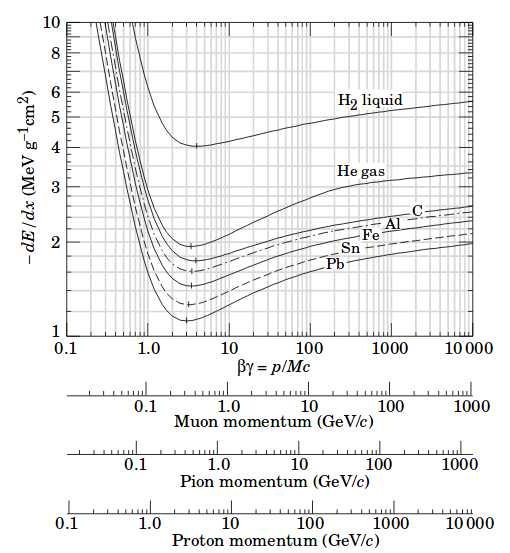
\includegraphics[width=0.50\textwidth]{images/PDGdEdX.png}
\caption{Mean energy loss in various materials over a range of particle momentums as produced in Reference \cite{PDG}.}
\label{fig:PDGEnergyLoss}
\end{figure}

Using the tables provided by the PDG for liquid argon (\cite{PDG-Argon}), we calculate the theoretical values for pions ($\pi$), muons ($\mu$), kaons ($k$) and protons ($p$) in the momentum range most relevant for LArIAT, shown in Figure \ref{fig:PDGEnergyLossArgon}. This prediction utilizes the Bethe-Bloch description of how much energy charged particles deposit corrected for the density using the Sternheimer parameterization. The most probable value is calculated as

\begin{equation}
\Delta_{p} (MPV) = \eta [ln (\frac{2 m_{e} c^2 \beta^{2} \gamma^{2}}{I}) + ln(\frac{\eta}{I}) + j - \beta^{2} - \delta(\beta \gamma)]
\end{equation}

where $\eta = \frac{1}{2} K z^2 \frac{Z x}{A \beta^2}$. Plotting $\Delta{p} / x$ shows the ``Fermi-Plateau'' for the various particles. A more in depth treatment of this function is given in \href{https://lartpc-docdb.fnal.gov/cgi-bin/private/RetrieveFile?docid=2567&filename=30June2017_Presentation_corrected.pdf&version=4}{docDB-2567}

\begin{figure}[htb]
\centering
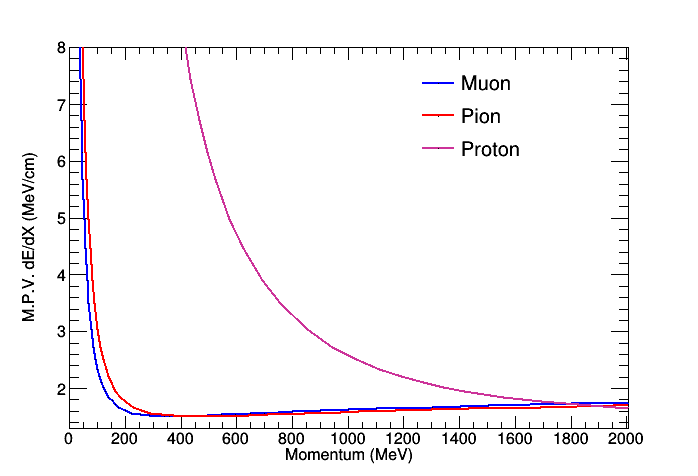
\includegraphics[width=0.60\textwidth]{images/dEdXvsMomentumTemplate}
\caption{Mean energy loss (solid line) and most probable value (dashed line) for pions, muons, kaons, and protons in liquid argon over the momentum range most relevant for LArIAT.}
\label{fig:PDGEnergyLossArgon}
\end{figure}

Using the predictions in Figure \ref{fig:PDGEnergyLossArgon}, allows us to tune the calorimetry constants used to convert the ADC to charge. The goal is to have the data and MC agree across the broad range of momentum. This tuning is done in addition to the wire-by-wire corrections (described in detail in \href{http://lartpc-docdb.fnal.gov:8080/cgi-bin/RetrieveFile?docid=1994&filename=investigation-uniformity-observed_v3.pdf&version=2}{doc-DB 1994}) and the usual lifetime corrections (described in detail in \href{http://lartpc-docdb.fnal.gov:8080/cgi-bin/ShowDocument?docid=1804}{docDB-1804}) which are used here and a more detailed treatment is left to their corresponding technical notes.

%%%%%%%%%%%%%%%%%%%%%%%%%%%%%%%%%%%%%%%%%%%%%%%%%%%%%%%%%%%
\subsection{Calibration Method Overview}\label{sec:MethodOverview}
%%%%%%%%%%%%%%%%%%%%%%%%%%%%%%%%%%%%%%%%%%%%%%%%%%%%%%%%%%%

Here describe the methodology used to select our samples and tune the calorimetry constants. Details specific to any one sample will be described in Section  \ref{sec:EventSelection} and we present the general method here and how it is applied. 

The basic idea of this calibration technique is to utilize a portion of a track within the LArTPC that has a well known momentum and particle species to measure the energy deposited per unit length (dE/dX) as recorded inside the TPC. Once a sample of particles dE/dX has been measured at various momentums, we then tune to calorimetry constants within the reconstruction software to align these measured values to match the theoretical ones found in Figure \ref{fig:PDGEnergyLossArgon}.

Since various electronics changes were done between Run-I and Run-II data taking periods, we derive calibration constants independently for both of these run periods. These calibration constants are the factors which convert the charge collected (dQ) to energy (dE). The details of how the calorimetry package works is beyond the scope of this note and is given in \href{http://lartpc-docdb.fnal.gov:8080/cgi-bin/ShowDocument?docid=2444}{docDB-2444}.

The calibration procedure follows the following basic steps:
\begin{itemize}

\item \textbf{Particle identification in the beamline:}

We first select a sample of beamline events that correspond to either a sample of $\pi, \mu, e$ or protons. This is done by selecting based on the measured time-of-flight (TOF) and momentum. 

For the calibration samples we require the tracks reconstructed in the wire chamber satisfy the criteria known as a ``picky track''. ``Picky tracks'' correspond to tracks reconstructed using hits in all four wire chambers. In these events, one and only one hit in each wire chamber track can be reconstructed per event and the track satisfies a straightness requirement in the Y-Z plane. These tracks have a more accurate measure of the particle momentum than the ``high yield'' tracks which only require hits in three out of four of the wire chamber tracks and can have mulitple wire chamber tracks reconstructed per event. Details about wire chamber track reconstruction can be found in \cite{WCTrackReco}

The wire chamber track is extrapolated to the front face of the LArTPC giving a $x, y$ position expected for the track in the TPC. A simple flat correction to the momentum as measured by the wire chambers due to the  energy loss by the particle as it traverses the material between the last wire chamber and the front face of the LArTPC is applied in data. 

For the Monte Carlo, no such beamline identification is done and instead we use the data-driven Monte Carlo (DDMC), which constructs the momentum and angular distributions for the single particle MC, and launches particles from the position of the fourth wire chamber (WC4) towards the TPC. We utilize the Monte Carlo truth for the position and momentum of the Monte Carlo particles as they enter the TPC.

\item \textbf{Matching LArTPC tracks to the wire chamber tracks:}

For each track reconstructed inside the TPC, the most upstream trajectory point (smallest $z$ position) is found. For that point we have it's $x, y, z$ as well as the calculated $p_{x}, p_{y}, and p_{z}$ (which is used to calculate the tracks $\theta, \phi$. Using this as well as the wire chamber tracks extrapolated $x, y, \theta, \phi$ we then select the event if there is one and only one TPC track which matches the wire chamber track. The exact matching criteria is given in Section \ref{sec:EventSelection}.

We now have the initial momentum (corrected for energy loss due to the upstream material) of the TPC track which we can use for our calibration. For the Monte Carlo, the ``wire chamber'' matching is done treating the true position of the MC particle as it enters the TPC as the ``wire chamber'' track. The rest of the matching proceeds just as before.

\item \textbf{dE/dX sampling:}

With the track within the TPC identified and the momentum for that track measured, we require the track to be of a minimum length of 10~cm long (to ensure we are away from any interaction point where the track may be broken into subsequent tracks). We then take the first twelve spacepoints of the track (excluding the first point to avoid edge effects near the field cage) and sample the reconstructed dE/dX for each point along the track. On average, this samples 5~cm of the track (shown in Section \ref{sec:Results}). These dE/dX measurments are then put into a histogram that corresponds to measured momentum of the track.

The dE/dX histograms are sampled every 50 MeV in momentum (e.g. 150~MeV $< P <$ 200~MeV, 200~MeV $< P <$ 250~MeV, etc...). On average, pions and muons only lose $\sim$10 MeV in this 5~cm section of the track and protons lose $\sim$20 MeV. Thus choosing 50 MeV size bins for our histograms should more than cover the energy spread within those bins due to energy loss from ionization.

This process of selecting, sampling, and recording the dE/dX for various momentum bins is now repeated over the entire sample of events, allowing us to collect sufficient statistic in most of the momentum bins between 150~MeV and 1100~MeV (which varies slightly, depending on the initial momentum spectrum for a given run period).

\item \textbf{Fit, tune, repeat:}

Each 50 MeV momentum binned dE/dX histogram is now fit with a simple Landau function. The fit range for the pion/muon sample is between 1.0 MeV and 5.0 MeV (bounds chosen to avoid the low dE/dX fluctuations seen in Run-1) and 2.5 MeV and 8.0 MeV for the proton sample. The most probable value (MPV) and the associated error on the MPV from the fit are extracted and plotted on Figure \ref{fig:PDGEnergyLossArgon}.

Depending on the outcome of the fit, the calorimetry constants are either tuned up or down. As a rule of thumb, if the returned MPVs are too high (meaning the fitted dE/dX is above the line), the calorimetry constants are increased (as counter intuitive as this seems...it is how its done). This both shifts the mean as well as changes the shape (since the recombination factor is applied to the dE derived from the calorimetry constants). Likewise, if the values are low the calorimetry constants are decreased. 

The values are tuned for both the collection and induction plane to try to achieve the best match to the theoretical curve that we can. The exact match is left as a qualitative exercise and is not quantitatively evaluated. While the tuning of the induction plane was done, the results are not shown in the technical note because, for the purposes of the forthcoming analyses we will only use the collection plane.

In addition to these distributions, the cumulative dE/dX distribution is also plotted and fit with a Landau function to assess the overall dE/dX calibration for the sample. This procedure is illustrated in Figure \ref{fig:CalibrationExample}.

\end{itemize}

\begin{figure}[htb]
\centering
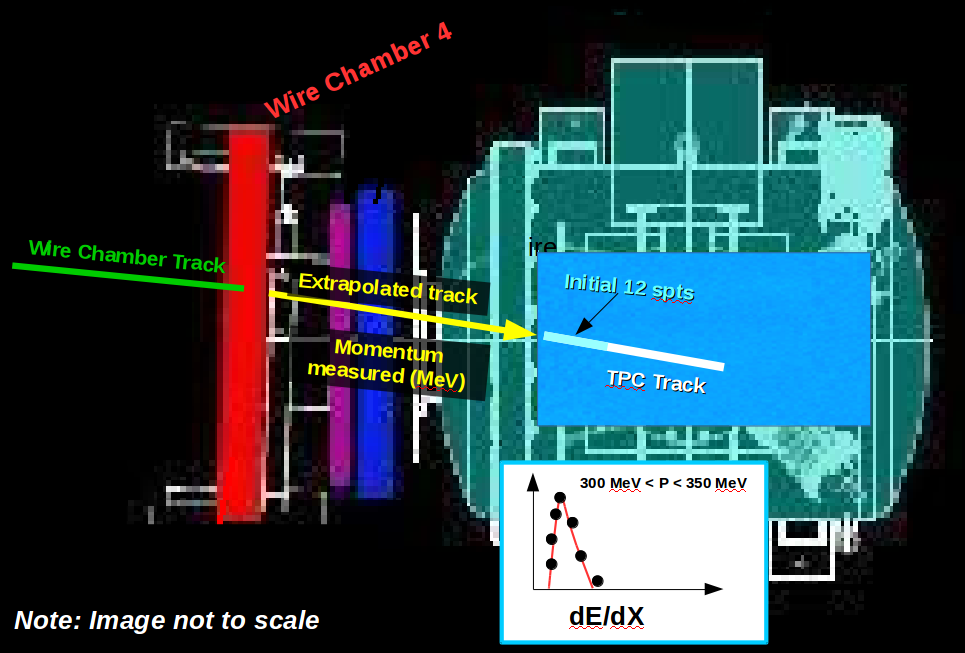
\includegraphics[width=0.50\textwidth]{images/CalibrationExample.png}
\caption{Illustration of the calibration technique. Here we depict a 325 MeV wire chamber track (shown in green) which enters the TPC (taking into account the energy loss from the upstream material) and we sample the first 12 spacepoints (shown in teal) to extract the dE/dX distribution which is fit with a Landau.}
\label{fig:CalibrationExample}
\end{figure}

With the procedure now laid out, we will move into the data and Monte Carlo samples used and the details of the event selection.
